
\documentclass{bigdata}
\newcommand\tab[1][1cm]{\hspace*{#1}}
\begin{document}
% Copyright
\setcopyright{acmcopyright}
%\setcopyright{acmlicensed}
%\setcopyright{rightsretained}
%\setcopyright{usgov}
%\setcopyright{usgovmixed}
%\setcopyright{cagov}
%\setcopyright{cagovmixed}
% DOI
\title{Tfidf in mapreduce and Testing YCSB\titlenote{d}}
\subtitle{Bigdata Project 2016,University of Trento}
\numberofauthors{1} 
\author{
\alignauthor
Tigist Abebaw Zeleke\\
              \email{abebawtigist@gmail.com}
}
\maketitle
%
% The code below should be generated by the tool at
% http://dl.acm.org/ccs.cfm
% Please copy and paste the code instead of the example below. 
%
\begin{CCSXML}
<ccs2012>
 <concept>
  <concept_id>10010520.10010553.10010562</concept_id>
  <concept_desc>Computer systems organization~Embedded systems</concept_desc>
  <concept_significance>500</concept_significance>
 </concept>
 <concept>
  <concept_id>10010520.10010575.10010755</concept_id>
  <concept_desc>Computer systems organization~Redundancy</concept_desc>
  <concept_significance>300</concept_significance>
 </concept>
 <concept>
  <concept_id>10010520.10010553.10010554</concept_id>
  <concept_desc>Computer systems organization~Robotics</concept_desc>
  <concept_significance>100</concept_significance>
 </concept>
 <concept>
  <concept_id>10003033.10003083.10003095</concept_id>
  <concept_desc>Networks~Network reliability</concept_desc>
  <concept_significance>100</concept_significance>
 </concept>
</ccs2012>  
\end{CCSXML}

%
% End generated code
%
%
%  Use this command to print the description
%
%\printccsdesc
% We no longer use \terms command
%\terms{Theory}
%\keywords{ACM proceedings; \LaTeX; text tagging}
\section{Introduction to the Problem}
\noindent
The focus of this work is divided in to parts one is to select mathematical algorithm and implement a serial and parallel implementation, The algorithm selected is TFIDF. TFIDF is a statistical measure used to evaluate how important a word is to a document in a collection or corpus. The Tf-idf weight is often used in information retrieval and text mining.  Tf-idf algorithm is often used in search engine, web data mining, text similarity computation and other applications. These applications are often faced with the massive data processing. So, how to calculate the tf-idf quickly and efficiently is very important. \cite{a} Search engines use it for scoring and ranking a document's relevance given a user query.\\
\noindent
In this project an illustration of implementation of the mathematical algorithm using Java is covered After that next is to implement the map-reduce parallel form using Hadoop map reduce Java API. And we see what the challenges of this method were and the solutions.\\
\noindent
The second part of the work is focused on experimenting with  Big Data technologies. In this project the problem of Benchmarking is selected. Hbase is selected for testing it. \\
\section{Related Work}
The papers that are reviewed are on the references.\cite{a},The implementation of map reduce algorithms are used by websites to check relevance of words. A term vector summarizes the most important words that occur in a document or a set of documents as a list of word, frequency pairs. The map function emits a host-name, term vector pair for each input document (where the host-name is extracted from the URL of the document). The reduce function is passed all per-document term vectors for a given host. It adds these term vectors together, throwing away infrequent terms, and then emits a final host name, term vector pair.\cite{b}. Some counter values are automatically maintained by the Map-reduce library, such as the number of in-put key/value pairs processed and the number of output key/value pairs produced.\cite{b}. \\

These paper reviewed shows a map-reduce pattern to improve TfIdf implementation using parallelization.\cite{a} In the mapper,  regular expressions are used to match words and write $<<word@documentName>, 1> $pairs to intermediate values which will be processed by reducer. Then we calculate the number of occurrences of the word in document directly in the reducer. The output of reducer need to be written to the intermediate files (tempFile1) which will be processed in next Map-reducer process.\\

Diffrent techniques from the book Mapreduce design Patterns \cite{c} have been reviewed. The tradeoff of being confined to the MapReduce framework is the ability to process your data with distributed computing, without having to deal with concurrency, robustness, scale, and other common challenges. But with a unique system and a unique way of problem solving, come unique design patterns.\\
\section{Problem Statment}
\noindent
TF-IDF weighting which stands for Term Frequency Inverse Document Frequency, The term frequency that shows the value of the word in a document that is in a corpus or collection. But has a inverse effect if the word is found in many documents. Thus the inverse document frequency. This is used to eliminate common words from appearing relevant. The IDF is logarithmically scaled.\\
The formula is as follows
\begin{equation}
w_{ij} = tf_{ij} idf_i = \frac{t_i}{d_j log(\frac{N}{n_i})}
\end{equation}
\noindent
In this work I have to find the TFIDF value for each  unique term in the document corpus.  The result of the matrix can be used later for data mining such as latent semantic analysis purposes another time. The corpus selected is the NSF dataset from http://archive.ics.uci.edu/. This data set consists of 129,000 abstracts describing NSF awards for basic research,it is totally 473 MB.  A web crawler is created to scrape the data from the website and put it in the user HDFS in one folder.
\\
\section{Solution}
\noindent
\subsection{Serial Version}
First the serial version needs to be computed to find a base for doing the parallel computation. It is a rather foreword implementation. When testing , this code took too much time to complete the work. Since the data the data is  large. 
\\
Algorithm: File Input\\
For each text file in the corpus\\
\tab For Each term in a Text-file\\
\tab \tab Put each term in Array string\\
\tab \tab Update Unique terms array\\
\tab Put each Array String in a  Array List\\

Algorithm: TFIDF\\
For each text files as Final Array List\\
\tab For each unique terms Array\\
TFIDF= TF(Text File Array, Unique terms)*\\
IDF(Text Corpus Array List, Unique terms )\\

Algorithm: TF\\
Compare each term in the text file with unique terms\\
 Count occurrence\\
 
 Algorithm: IDF\\
 Compare each term in the corpus with unique terms\\
 Count occurrence and do Inverse calculation\\
\subsection{Parallel Version}
\subsubsection{Implemented Solution}
Here I discuss the implementation and comparison with an already implemented solution by marcellodesales on His website. The implemented solution is as follows. It is tested on hadoop-2.5.0-cdh5.3.2 environment on HDFS. The next step is to change the above algorithm to a map-reduce parallel implementation. To so this implementaition I used some of the guide lines from the paper , Improvement of TF-IDF Algorithm Based on Hadoop Framework \cite{a}. The system that is used  for implementation is the Apache Hadoop /HDFS Ecosystem. Hadoop provides a distributed file system and a frame work for the analysis and transformation of very large data sets using the MapReduce paradigm.\cite{d}.The HDFS architecture is divided in to name nodes and Datanodes, The name node contains the mapping of file blocks location to Data-nodes. Datanode contains the data itself and the metadata. HDFS is different from other file systems  , that is provides an API that exposes the location of file blocks. This allows the map-reduce frame work to give task on the data location which improves read performance.\\

The Map-reduce Algorithm forms the input as Key/Value pairs, user creates a Map function to divide the task in to smaller tasks that will do a grouping based on an intermediate key. The reducer merges the above values. One way to do it would be to find the TF Job on the document. Process the IDF Job of The same document. But this will double the computation. So passing the result of the TF to the IDF as arguments is better choice. TF Job writes in to a file outputTF which becomes input for IDF jOB. The problem here is How can we pass the input arguments using formats like Text, LongWritable. \\

The solution is to have a customized IO class, that is to extend the FileInputFormat <Text, IntWritable> class together with RecordReader <Text, IntWritable>. From the file, But reading every line as string separated by tabs from it converts it to a Text, Intwritable format suitable for mapping. Similary after the IDF Job is done it passes arguuments to TFIDF class . Here We need both text inputs as Key and value so we extend the FileInputFormat <Text, Text>,RecordReader <Text,Text> instead. 
Another method used is since we have only <key,value> pairs, How can we pass more than two parameters. The solution is to use $“_”$ separated strings. The TFIDF reducer doesnt do counting or summerization but does ouputing the tfidf values together with the term.\\
\\
Algorithm\\
TF \\
Mapper<object, Text, Text, Intwrittable>\\
      \tab <term, one>\\
Reducer<Text, Intwrittable,Text, Intwrittable>\\
     \tab   $<docCode_term, frequency>$\\
\noindent       
IDF\\
Mapper<Text, IntWritable, Text, Text> \\
     \tab   $<term, docCode_termFreq>$\\
Reducer<Text, Text, Text, Text>\\
    \tab    $<term, docCount_docId_countInDoc>$\\
TFIDF\\
Mapper<Text, Text, Text, DoubleWritable>\\
     \tab    $<noDocterm_docCode_termsInDoc[1]_key, tfidf[1]>$\\
Reducer<Text, DoubleWritable, Text, DoubleWritable>\\
        <key,tfidf>\\
        
The agreggator class combines the three jobs together. It is unable to take the HDFS as input , unless the path to the HDFS is hard coded. Which is not coonvinient, so it is left as it is. After the output runs it stops after doing only outputTF.The solution is to have three separate jobs , If it is necessary to check it on HDFS,Instead of the agregator job which does runs the tf,idf,TfIdf jobs automatically. The solution is to make it read Input from the output directory on HDFS. From the local system it works without such issues. So a different run.sh is provided.
The main Lesson learned here is. When coming up with a map-reduce algorithm it is not necessary to follow the serial version, It has its own new ways that makes it simpler and efficient. It is a different paradigm. 
\subsubsection{Comparison}
Among the implementations by others on this same problem I will discuss the one of implementation by TfIdf in Hadoop.Our modeling for the <Key,Value> pairing is almost similar to his modeling as well as the method of using the result of each job as intermediate values for the next jobs is also similar. https://marcellodesales.wordpress.com. \cite{d}. The following is taken from his website.\\

In order to decrease the payload received by reducers, I'm considering the very-high-frequency words such as "the" as the Google's stopwords list.
Aside from Diffrence in the technical programming.He has used  Test-Driven Development , he implemented a mapper unit test an a reducer unit test. Before executing the hadoop application,to let the Mapper and Reducer classes to pass to the the unit tests. It is mentioned that this helps during the development of the Mappers and Reducers by identifying problems related to incorrect inherited methods (Generics in special), where wrong “map” or “reduce” method signatures may lead to skipping designed phases. Therefore, running the test cases before the actual execution of the driver classes is safer. \\
Inour case it is implemented a diffrent Input class to data format the IDF parameters in the necessary way. In his case , he has implemented a String manipution to get the necessary <key,value>  datatype formating inside the mapper, after the parameters are already retrieved exactly as they are passed.\\

TF\\
\tab    Map:\\
\tab \tab       Input: (document, each line contents)\\
\tab \tab       Output: (word@document, 1))\\
\tab    Reducer\\
\tab \tab      n = sum of the values of for each key “word@document”\\
\tab \tab       Output: ((word@document), n)\\
\tab    Map:\\
\tab \tab        Input: ((word@document), n)\\
\tab \tab Re-arrange the mapper to have the key based on each document\\
\tab \tab        Output: (document, word=n)\\
\tab   Reducer\\
\tab \tab        N = totalWordsInDoc = sum [word=n]) for each document\\
\tab \tab        Output: ((word@document), (n/N))\\
\tab     Map:\\
\tab \tab        Input: ((term@document), n/N)\\
\tab \tab        Re-arrange the mapper to have the word as the key, since we need to count \tab \tab the number of documents where it occurs
\tab \tab        Output: (term, document=n/N)\\
\tab   Reducer:\\
\tab \tab        D = total number of documents in corpus. This can be passed by the driver \tab \tab as a constant;\\
\tab \tab        d = number of documents in corpus where the term appears. It is a counter  \tab \tab over the reduced values for each term;\\
\tab \tab        TFIDF = n/N * log(D/d);\\
\tab \tab        Output: ((word@document), d/D, (n/N), TFIDF)\\
Solution:\\
InputSplit\\
InputSplit represents the data to be processed by an individual Mapper.
Typically InputSplit presents a byte-oriented view of the input, and it is the responsibility of RecordReader to process and present a record-oriented view.
FileSplit is the default InputSplit. It sets mapreduce.map.input.file to the path of the input file for the logical split.\\

RecordReader\\
RecordReader reads <key, value> pairs from an InputSplit.
Typically the RecordReader converts the byte-oriented view of the input, provided by the InputSplit, and presents a record-oriented to the Mapper implementations for processing. RecordReader thus assumes the responsibility of processing record boundaries and presents the tasks with keys and values.\\
The results are similar to the Figures below.
\begin{figure*}
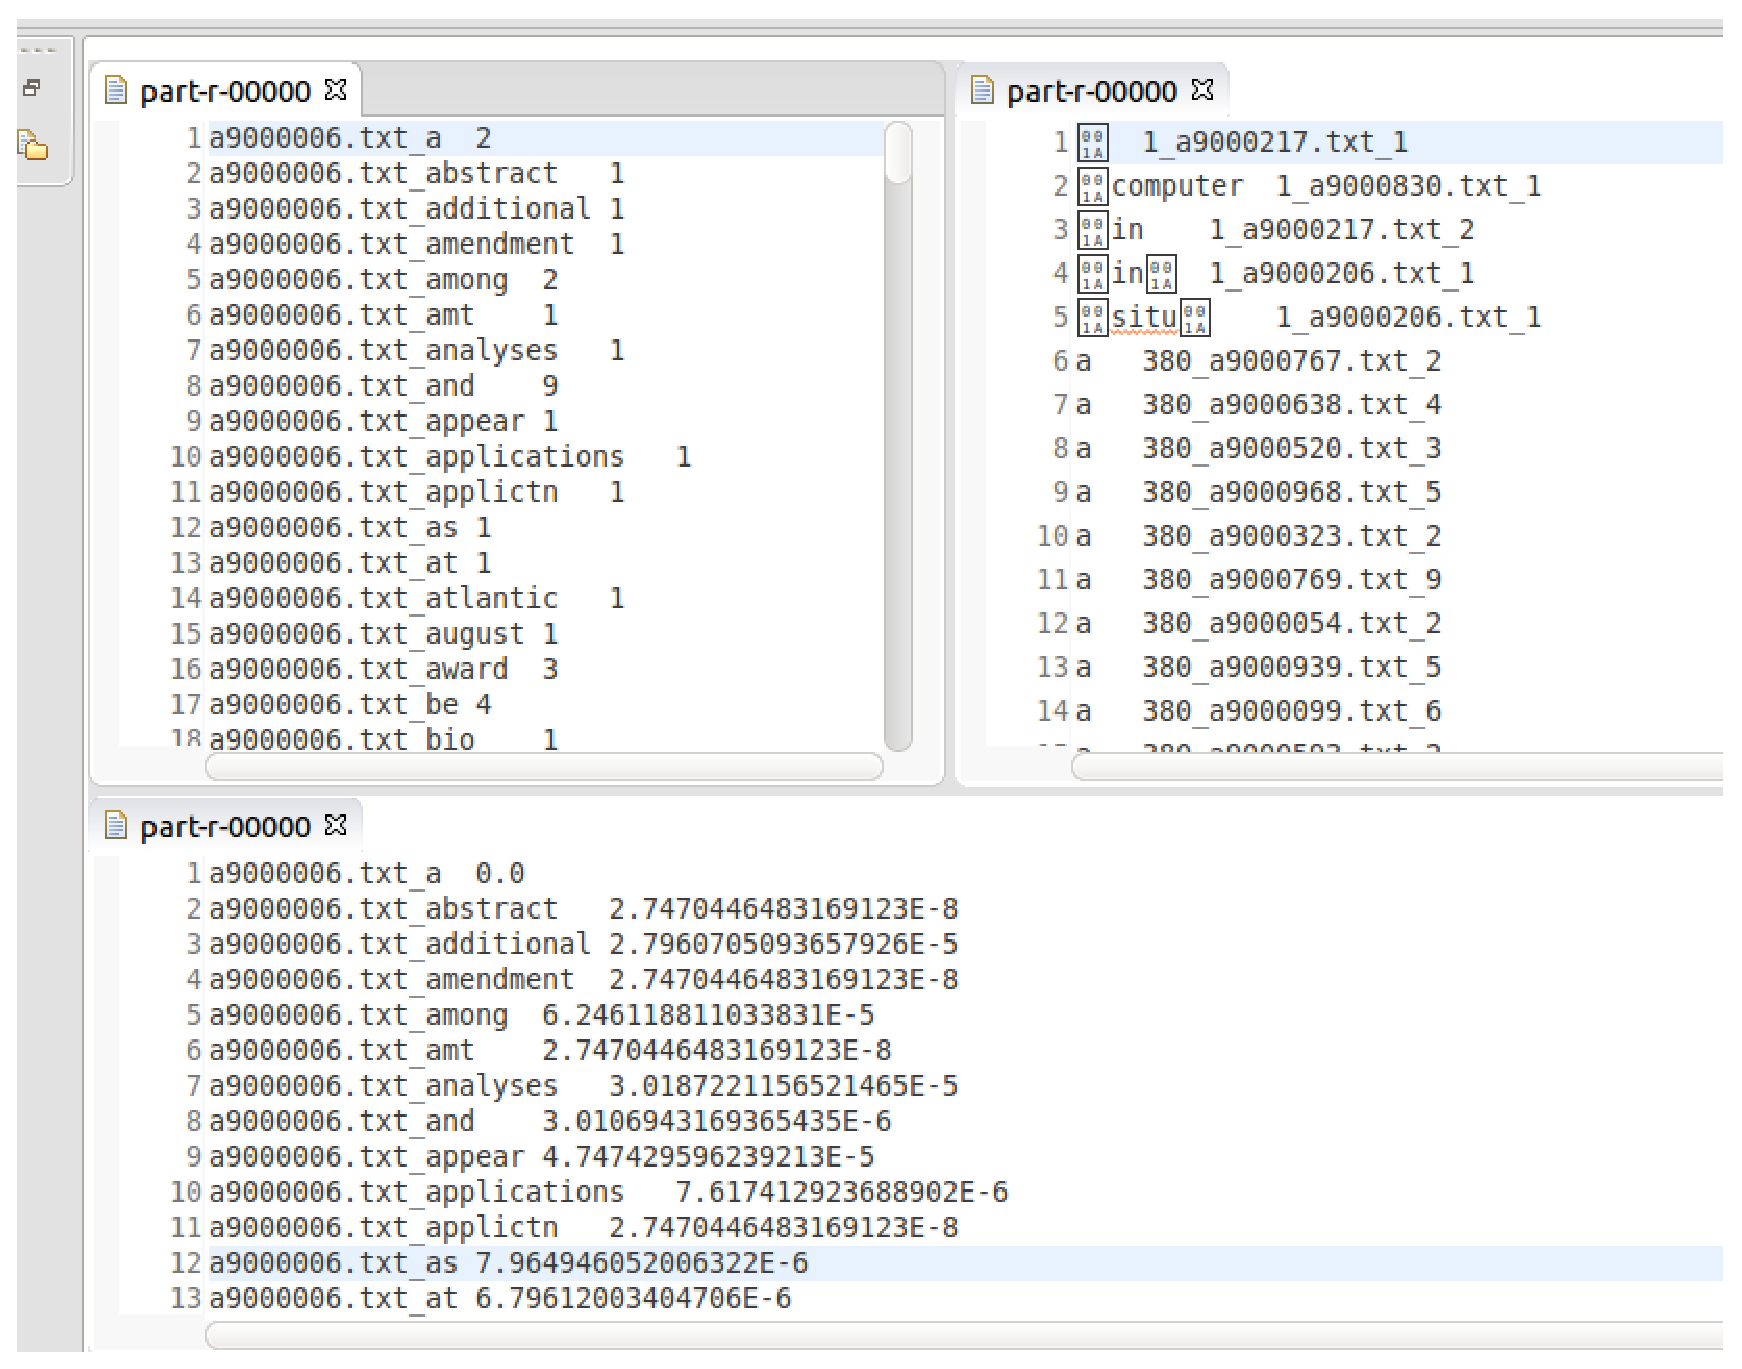
\includegraphics[height=6in, width=6in]{image4}
\caption{Right TF, Left IDF, Bottom TFIDF results}
\end{figure*}
\section{Experiments}
I have selected the problem of Benchmarking using Yahoo!'s YCSB Benchmarking technique for experimentation on Hbase in particular. After setting up Hbase clustered mode.Benchmarking is the process of running a a number of standard tests on a set of computer programs.\\

Database bench marking involves simulations of tests on varying workloads  varying data volumes and specific queries tuned or by changing hardware configurations and database configuration setting. It is used to compare versions of different databases or among diffrent databases. Its significance is valuable for complex and large scale systems. Here we will see how we can use benchmarking suit in order to get results when we want to analyse our key-value storage.\\

Large scale databases have difference of data model. Such as column oriented or document model. With the continuous growth of enterprise systems, sometimes extending over multiple data centers, and the need to track and report more detailed information, that has to be stored for longer periods of time, a centralized storage philosophy is no longer viable. \cite{g} Because of these requirements, emerging storage systems have to be explored in order to develop an APM(Application Performance Management) platform for monitoring big data with a tight resource budget and fast response time. \\

There are built in benchmarks in databases or third party customized benchmarking tools. such as the MySQL\\ BENCHMARK($loop_count$,expression). Also there are load testing and benchmarking tools for relational databases such as  Oracle Database, Microsoft SQL Server, IBM DB2,  MySQL, PostgreSQL and others. One is HammerDB for relational DB. For no sql databases the YCSB Benchmark suite that can be used for testing the performance of key-value stores. \\
It is difficult to test different storages and compare them. Moreover, an apples-to-apples comparison is hard, given numbers for different systems based on different workloads. Thus, developers often have to download and manually evaluate different systems. \cite{f}\\
YCSB Yahoo Cloud serving benchmarking framework is developed to assist with this issue.  There are common workloads that come with the frame work included. It is extensible so that developers can define their own workloads. To compare the results plotting can be used. \\
When we compare among diffrent cloud storage systems we take in to consideration their properties.Mainly they have three common designs. They are designed to Scale out which is  to avoid bottle necks and balance loads across servers.  Elasticity which is to add new instances and loads to them. And high availability , to be able to recover from failure.Inorder to achieve these on a real hardware the systems manage their own tradeoffs.\\
Read performance versus write performance,to read from large storages. Random I/O will be used since all data can not fit in the memory. Log-structured merge trees \cite{f} trade-off between optimizing for reads and optimizing for writes\cite{f}. Latency versus durability is the other one. Latency performance can be improved if writes are done on a memory temporarily. But there is a risk of data loss in-case of system failure. Synchronous versus asynchronous replication. where, availability may be impacted if synchronously replicated updates cannot complete while some replicas are
offline. Asynchronous replication avoids high write latency but allows replicas to be stale. Furthermore, data loss may
occur if an update is lost due to failure before it can be
replicated.\\
We believe an industry standard big data benchmark must be an end-to-end benchmark\cite{h} covering all major characteristics in the life cycle of a big data system including the three(I) volume (larger data set sizes), (ii) velocity (higher data arrival rates, such as click streams) and (iii) variety (increased data type disparity, such as structured data from relational tables, semi-structured data from key-value web clicks and UN-structured data from social media content)\cite{h}
\subsection{Types of tests}
The YCSB Benchmarking will be done on Hbase storage system.It has a data generator and a workload generator.It is written in Java is programmed to load data to data system and perform operations called workloads. It tries to check the performace characteristics disscussed above. And reports the statistical Results.I will use the core workloads a-f on Hbase.System Property. The work loads include funcions to simulate the crud operations read, insert,update, delete and scan operations.For example workload a which is shown below.\\
Although bench marking is performed on a largedata system with multiple clusters to get real results. This experimentation is to do a simple comparison of the effects of the workloads. One issue found during implementation of region servers was that YCSB used its own port. And zookeeper uses ports to manage region servers. And this has caused a conflict error.Unable to find znode. But after diffrent trials it was not able to be solved.  So the test was done on master node.And  64-bit intel core i7 2.40GHz*4 Intel Xeon CPUs, 7.7 GiB of RAM, 467.8 GB disk. With hadoop-2.5.0-cdh5.3.2 and Hbase 0.98.8 and YCSB 9.0 Hbase 1.0.x binding.\\
....
Workload a\\
recordcount=1000\\
operationcount=1000\\
readallfields=true\\
readproportion=0.5\\
updateproportion=0.5\\
scanproportion=0\\
insertproportion=0...

Hbase is a column oriented database management system. Since it does not use relational query language like SQL. Its programs are written as mapreduce on java. An Hbase table is accessed using its primary key. It stores column families that are with common attributes. But column families can be added at anytime. It hase a mastor node and region servers. It is able to store large tables. It is convinient to store sparse data. It has the following properties. Replication, high availability, in memory caching and real time processing. 
\subsection{Results}
After running Hadoop and Hbase, we run the YCSB workloada which loads only 1000 records to check on read and update operations based on the above snippet of code from coreworkloads. The results can be seen on fig Reference.. show that the total excecution time for loading the data is 3209.0 sec,  it has a through put of 311.6 operations/ sec and an avarage latency of 2015.0 sec.

 Then the next step is to run the operation in this case read and update.It is 50 percent read and 50 percent update.  That means on half of the data, 483.0 read operations.It is given 10 threads and 50 operations per sec as target. The result was an average latency of 30888.6 operations per sec. Where as the overall throughput of the run was 47.2 operations per second. And also results for update can be seen. As latency which is the time to do a single operation increases the through put that is the number of operations per time period decreases and a good system must be able to balance it.  

Inaddition editing of workloads is done to check extensibility. Changing records to 10000 and was able to get results as expected, so in the future to do better analysis Increase in number of records was done to 10000.



\begin{figure}
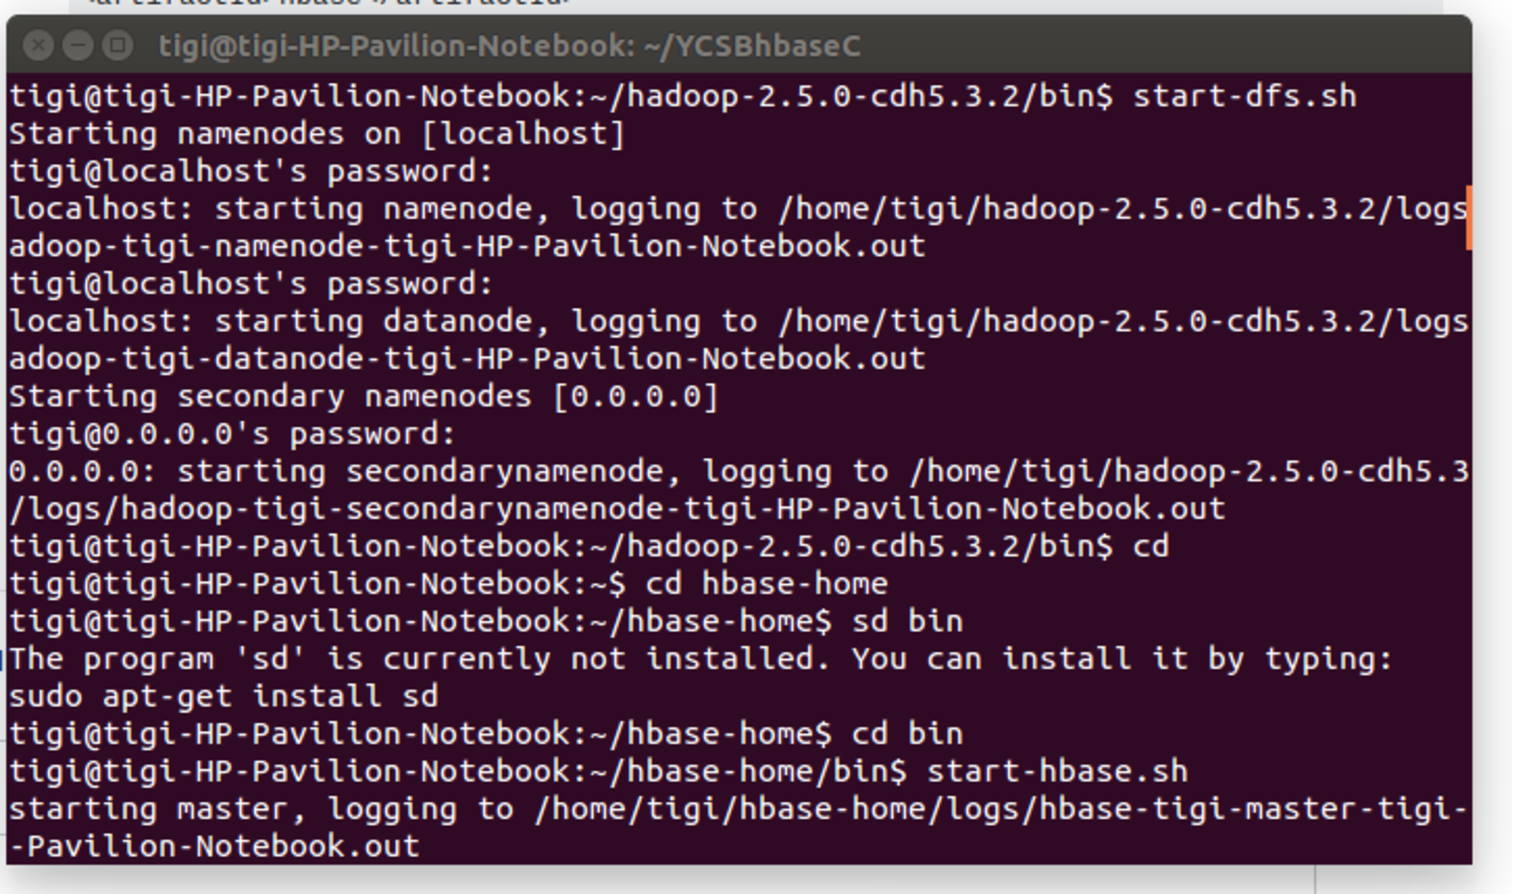
\includegraphics[height=3in, width=3.5in]{image2}
\caption{Starting Hadoop and Hbase}
\end{figure}
\begin{figure}
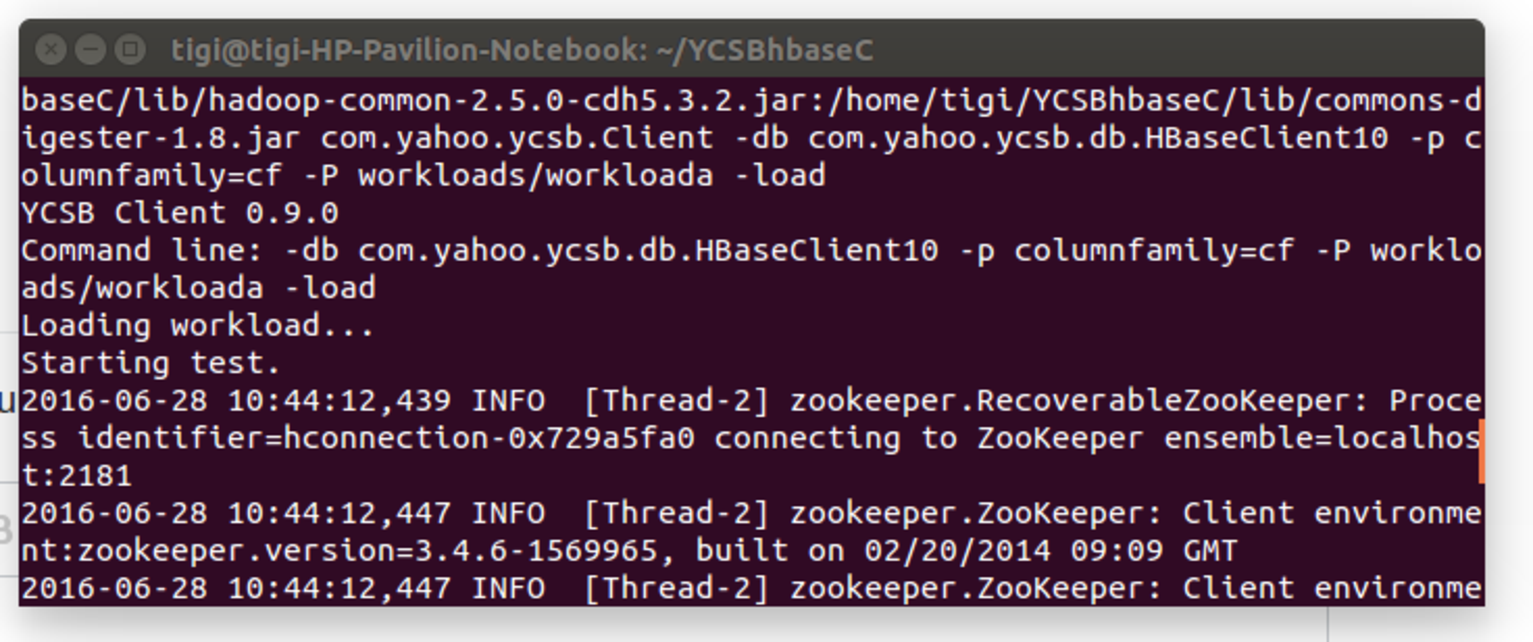
\includegraphics[height=3in, width=3.5in]{image1}
\caption{Starting the Test}
\end{figure}
\begin{figure}
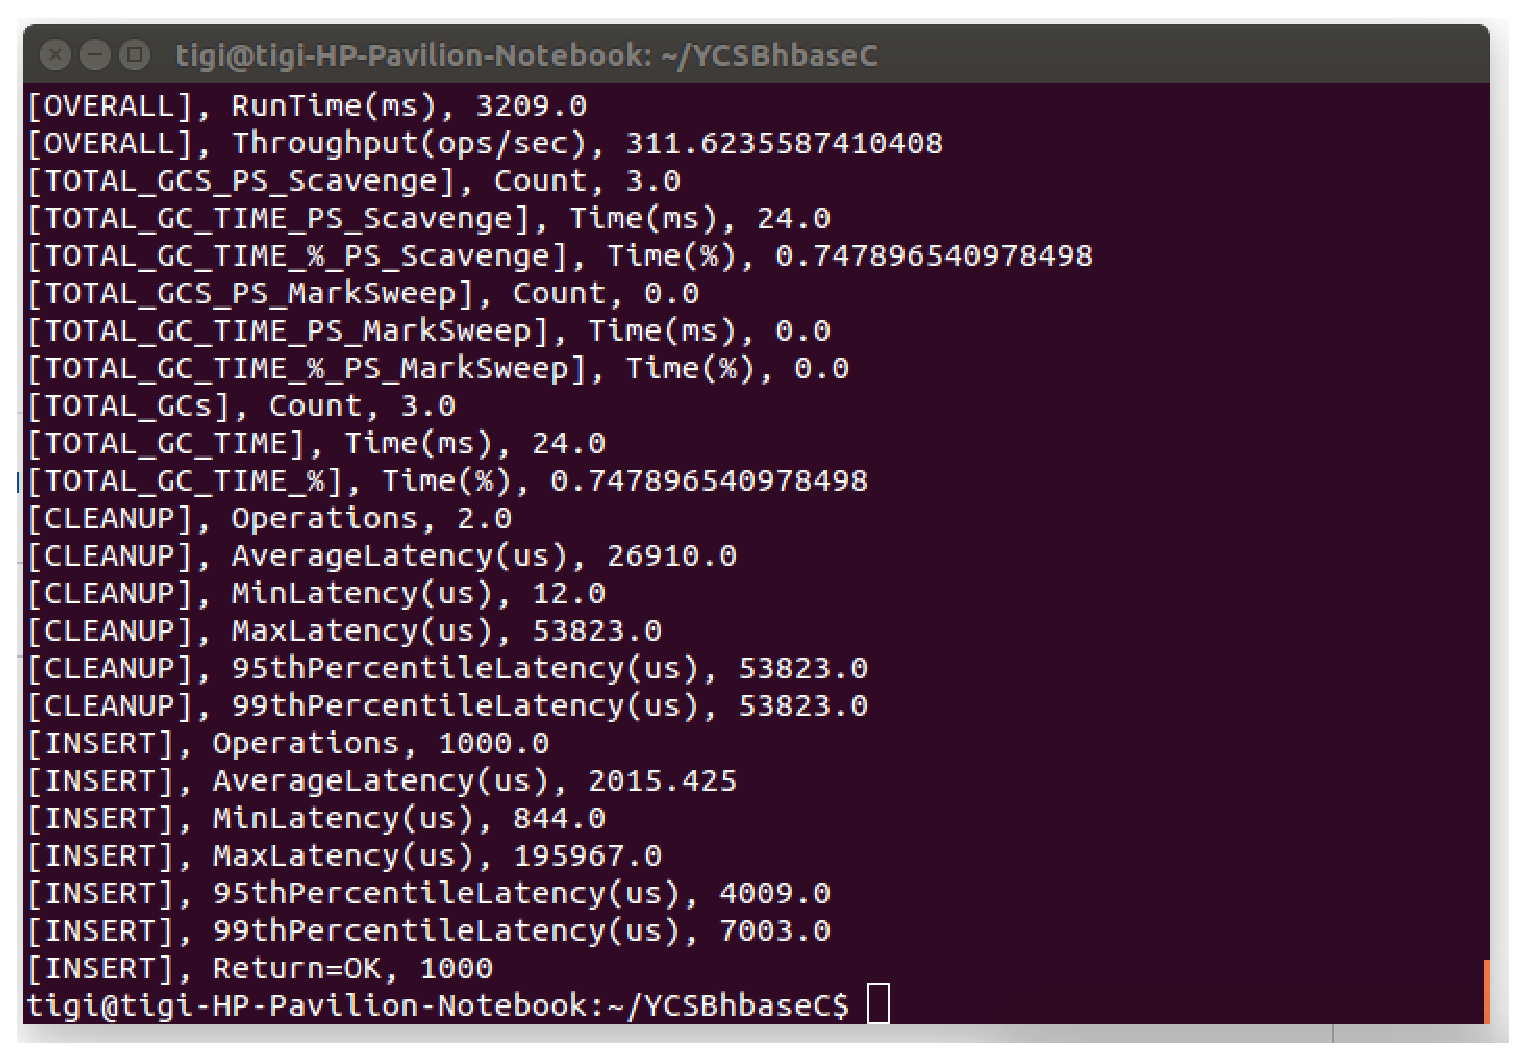
\includegraphics[height=3in, width=3.5in]{image3}
\caption{Result of Workload a Load data  for 1000 Records}
\end{figure}
\begin{figure}
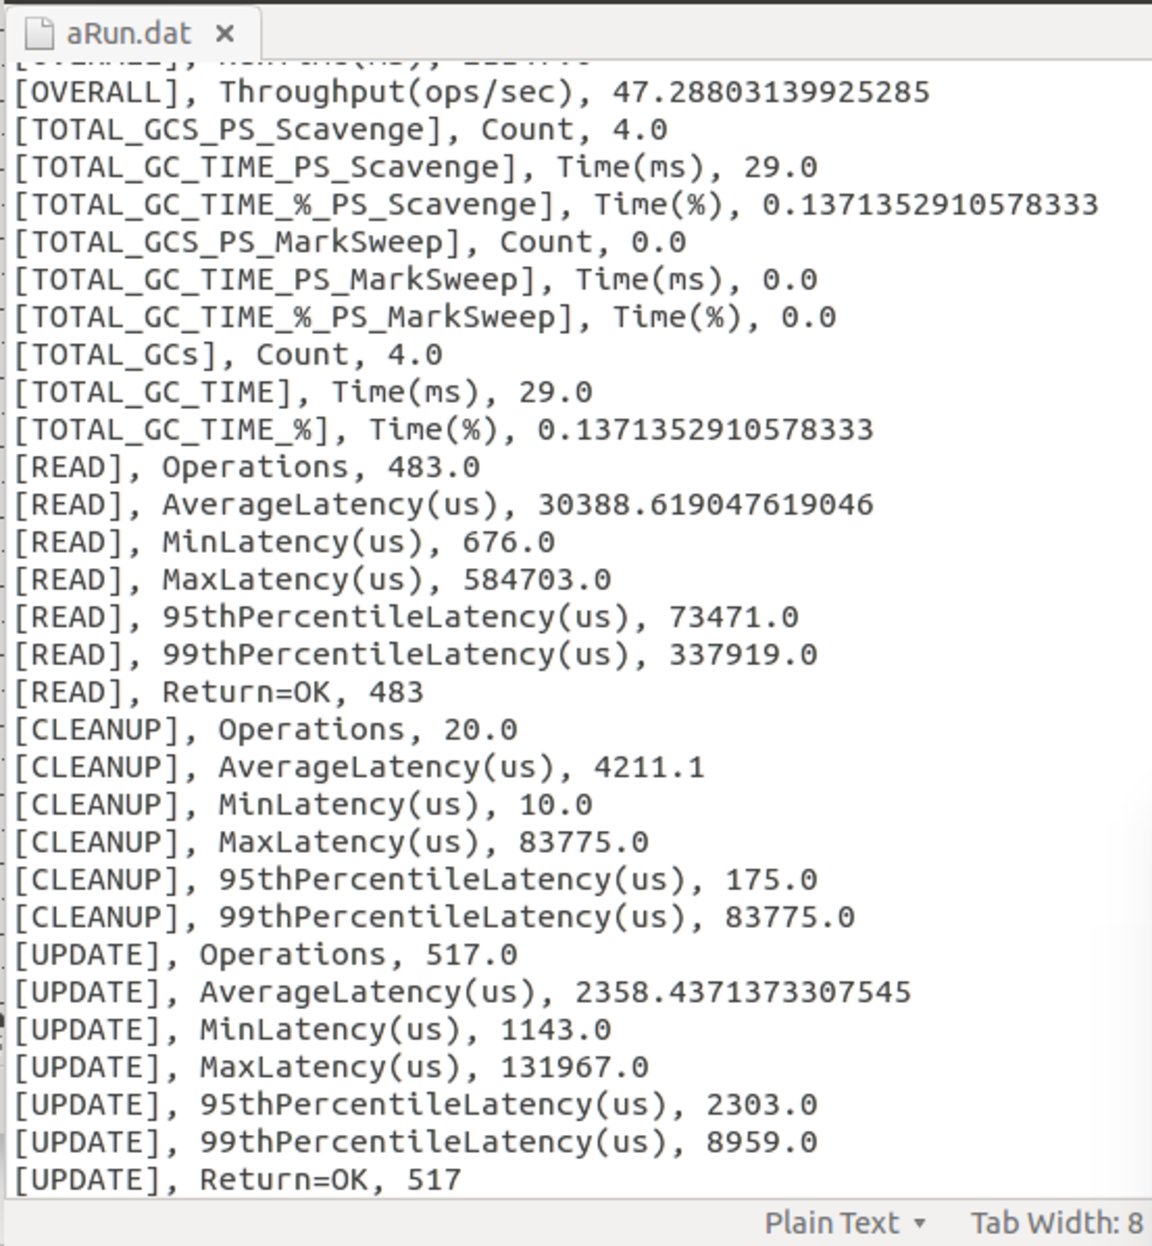
\includegraphics[height=3in, width=3.5in]{image5}
\caption{Result of Workload a Run data for 1000 Records}
\end{figure}


%\end{document}  % This is where a 'short' article might terminate
%
% The following two commands are all you need in the
% initial runs of your .tex file to
% produce the bibliography for the citations in your paper.
\bibliographystyle{abbrv}
\bibliography{sigproc}  % sigproc.bib is the name of the Bibliography in this case
% You must have a proper ".bib" file
%  and remember to run:
% latex bibtex latex latex
% to resolve all references
%
% ACM needs 'a single self-contained file'!
%
%APPENDICES are optional
%\balancecolumns
\end{document}
